Voxie supports the creation of slices. A slice is a plain intersecting the dataset. 
Its visual representation is defined by all voxel values it intersects.

Voxie supports multiple operations on slices. This includes adjusting, filtering, colorizing and analyzing.

\subsubsection{Creating a slice}

A slice is created by telling the data set (VoxelData) to create a new slice. In the UI this is done by clicking on the \textit{Create Slice} button in the section representing the data set.

After adding a slice a new section will appear displaying the position and rotation of the slice. The 3D image describes the position of the slice within the dataset. Values are coded as x (green),  y (blue), z (red). The rotation is displayed as normalized quaternion.

\begin{figure}[h]
	\caption{Slice Section}
	\centering
	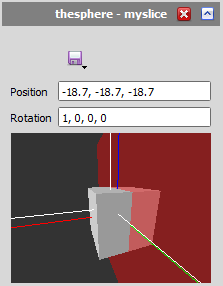
\includegraphics[scale=1.0]{img/2d/3dslice.png}
\end{figure}

\subsubsection{Exporting a slice}

The raw values of the slice can be exported in HDF5 format by clicking on the \textit{Save} button in the slice's section.

\subsubsection{Displaying a slice}

To display a slice Voxie's SliceView plugin has to be used. To add a new Slice View click on Visualizer, then 2D, then Slice.

A dialog will appear. Choosing a slice will create a new window and several new sections.

\begin{figure}[h]
	\caption{The Slice View and its sections and tools}
	\centering
	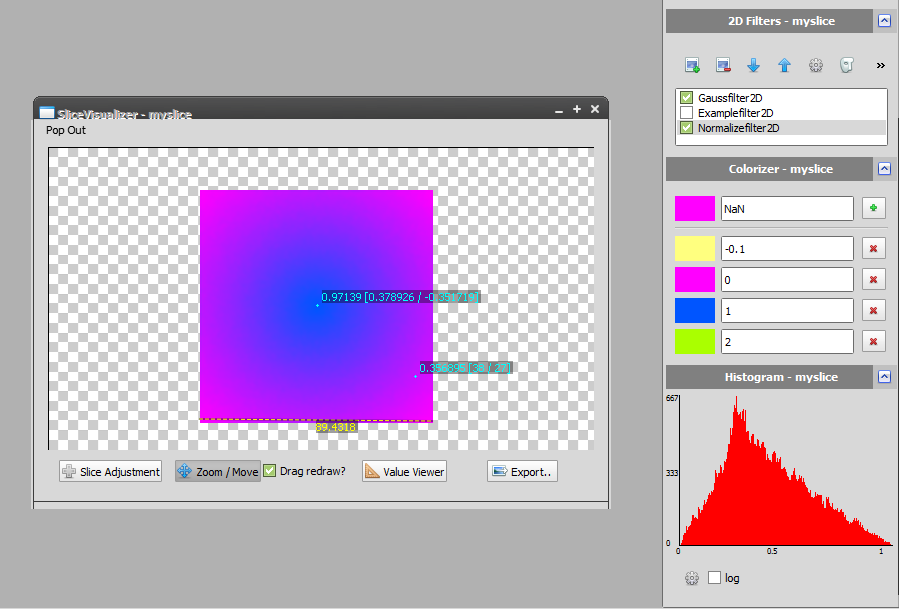
\includegraphics[width=1.0\textwidth]{img/2d/sliceview.png}
\end{figure}


\subsubsection{The slice view}

By default the slice view window offers a canvas that displays the slice associated with the slice view. It also allows for tools to be used which can modify the slice or display information. Tools can be switched by using the number keys.

\subsubsection{Slice Adjustment Tool}
The slice adjustment tool allows for interactive adjustments to be made to the slices configuration.
When this tool is active the x and y axis of the slice are shown (x = green , y = blue). Notice that x points
right and y points down(!).
\\ \\
The slice's origin can be moved to another point on the plane by [right-clicking]. This is useful because the slice's origin is the pivot point for its rotations.\\
The slice's origin can also be moved along its normal vector with the mouse-wheel or [page-up/down] keys. This
Movement can be fine adjusted by holding down [shift] simultaneously.
\\ \\
The slice's rotation can be adjusted an variuos ways.
To rotate the x-y-plane (rotate arround normal vector) hold down [ctrl] and [drag] the mouse with [left-click] arround the origin. \\
This way you can also rotate arround the other axes. To rotate the slice arround the x axis hold down [ctrl]+[x] and drag with [left-click], with [ctrl]+[y]+[left-click][drag] you can rotate arround the y axis. \\
Alternatively you can use the arrow keys [up]/[down]/[left]/[right] to rotate arround the x or y axis. [shift] can be used to slow down the movement with the arrow keys.
\\ \\
For more arbitrary rotation you can "push down" the slice on a specific point with a simple [left-click]. This causes the slice to tilt towards the direction of clicked point (origin is pivot point). To fully understand this imagine the vector that points from the origin to the click point, the vector that is perpendicular to this vector and the normal vector of the plane is the axis of rotation.\\
The step-size can be reduced by holding down [shift]. 

\subsubsection{Zoom / Move Tool}
The zoom and move tool allows one to zoom and move around the displayed image. Holding the left mouse button and dragging will move the image around. The mouse wheel is used to zoom the image. Toggling the checkbox labeled \textit{Drag redraw?} will allow for less processing power to be required as the image will only be altered when the mouse button is released.

\subsubsection{Value Viewer Tool}
The value viewer tool displays values within the image. The value shown below the curser represents the position and the float value of the slice at the given position. Left-clicking will make the value continue to be displayed. Right-clicking will clear all displayed information. Pressing shift shows the unfiltered value. Pressing control will round the position values. Dragging the mouse will calculate the distance between two points in metric distances (see HDF5 specification). Modifying the slice or the generated image will clear all values.

\subsubsection{Mask Selection Tool}
\label{sec:mask}
The Selection Tool allows the User to select an area on the image and on this selected area the filter is applied to. To use this function a filter in the Filter Chain must be selected and only on this filter the mask is applied on. To create a mask you have to click on the mask symbol, then four new buttons appears on the Slice View, \grqq Rectangle\grqq, \grqq Ellipse\grqq, \grqq Polygon\grqq and \grqq Clear\grqq.
\\[12pt]
By clicking on the \textbf{Rectangle Button}, it allows to create a rectangle shape. To do that click and hold the left mouse button and move the mouse. A yellow rectangle appears, this shows the preview of the selection. By realising the left mouse button it finishes the selection and the yellow rectangle turns into red.
\\[12pt]
By clicking on the \textbf{Ellipse Button}, it allows to create a ellipse shape. To do that click and hold the left mouse Button and move the mouse. A yellow ellipse appears, like before it shows the preview of the selection. The first click defines the center of the ellipse. By realising the left mouse button it finishes the selection and the yellow rectangle turns into red.
\\[12pt]
By clicking on the \textbf{Polygon Button}, it allows to create a polygon shape. To do that click on the image, every click is one vertex of the polygon. Every click connects the vertices in yellow, this is just the preview. By pressing space, the polygon shape closes automatically. Notice that at least three vertices are needed to close a polygon shape.
\\[12pt]
By clicking on the \textbf{Clear Button}, it deletes every created shape on the mask only for the selected filter.

\subsubsection{Export Tool}

The export tool will allow for the currently displayed image to be saved. There are three modes available; filtered image, filtered and colorized image or the whole canvas (including borders outside the image).

\subsubsection{Slice View Sections}

A slice view creates three new sections on initialization.

\begin{itemize}
	\item{\emph{2D Filter }\newline This section allows for definition of filters, their order and masks. An ordered set of filters is called a filterchain.}
	\item{\emph{Colorizer}\newline The colorizer section maps values to colors. In between values will be interpolated.}	
	\item{\emph{Histogram}\newline The value distribution is visualized here. It also offers advanced options like logarithmic scaling.}

\end{itemize}

\begin{figure}[h]
	\caption{2D Filter Section}
	\centering
	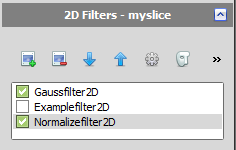
\includegraphics[scale=1.0]{img/2d/2dfilter.png}
\end{figure}

\subsubsection{Adding 2D Filters}

A 2D filter can be added by clicking on the \emph{Add Filter} button will open a dialogue allowing one to choose what kind of filter is to be added. Filters are automatically active after creation.

\subsubsection{Removing 2D Filters}

Filters can be removed by highlighting a filter in the section then clicking the \emph{Remove Filter} button.

\subsubsection{Choosing which Filters to apply}

Filters can be temporarily deactivated by toggling the checkbox next to their name.

\subsubsection{Ordering 2D Filters}

Filters are applied in order from top to bottom. Their ordering can be altered by highlighting a filter then pressing the array buttons to move them up or down.

\subsubsection{Configuration of 2D Filters}

Some filters posses a configuration dialogue. The dialogue can be opened by highlighting the desired filter then pressing the \emph{Options} button (\emph{Wheel}).

\subsubsection{Loading and saving Filterchains}

Filterchains including the individual filter settings can be exported and imported using the \emph{Export Filterchain} and \emph{Import Filterchain} buttons. The filterchain will be represented by a human readable xml file.

\subsubsection{Filter Masks}

After activating the filter feature by adding filters, the \emph{Filter Mask} button will activate the filter mask feature in the slice view. This allows for the \emph{Mask Selection Tool} to be used. See \ref{sec:mask} for more information.

\begin{figure}[h!]
	\caption{Colorizer Section}
	\centering
	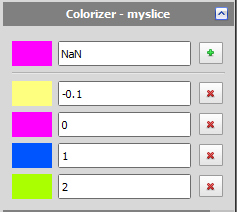
\includegraphics[scale=1.0]{img/2d/colorizer.png}
\end{figure}

\subsubsection{Colorizer}

The colorizer maps values to colors. Colors in between the given mappings will be interpolated. Mapping can be added by pressing the \emph{Add Mapping} button in the first column. This will add a new mapping to the list of mappings below.\newline The colors can be changed by clicking on the displayed color. This will invoke the operating system specific color picker. \newline To remove a mapping simply click on the \emph{Remove Mapping} button. \newline Please note that mappings with the same value will be automatically merged, the new mapping having priority.

\subsubsection{Histogram}

The histogram section shows a visualization of the value distribution of the slice. The scale can be set to be linear or logarithmic. Upper and lower bound as well as the maximum count value can be set via dialogue.
 
\subsubsection{Displaying the difference between two slices}

If two Slices should be compared, the DiffView plugin has to be used. To add a new DIff View click on Visualizer, then 2D, then DiffView.

A dialog will appear. Choosing two slices will create a new window and several new sections.

The DiffView is build similar to the SliceView, thereforce the following subsctions only describe the changes between the DiffView and the SliceView.


\subsubsection{Slice Adjustment Tool}

The Slice Adjustment Tool within the DiffView brings two new buttons: "Switch Slice" to switch the slice that is currently adjusted and "Select Both" to adjust both slices at the same time.

The Origin of the currently not altered Slice will be shown as DashLine. 

\subsubsection{Value Viewer Tool}
The value viewer for the DiffView will always display two values, as there are two Slices, except if the Shift-Key is pressed, then the value for the filtered Image (which is not connected to a slice anymore) will be shown.
